\chapter{Split-Cylinder Resonator}\label{ch:splitc}
\begin{figure}
\centering
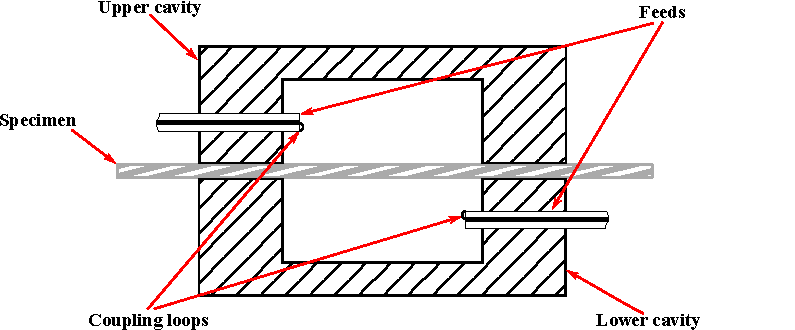
\includegraphics[width=0.8\textwidth]{split_cylinder_resonator.pdf}
\caption{Split-cylinder resonator.}\label{fig:split_cyl}
\end{figure}
In the previous chapters of this thesis we have now covered the fundamentals of permittivity and dielectrics, the dielectric measurement methods at microwave frequencies and the theory of quality factor measurements, but we have not touched the main topic of this thesis, the split-cylinder resonator. Like the resonators mentioned in Chapter \ref{ch:methods}, the split-cylinder resonator is a dielectric measurement method of the standing-wave type. As can be seen in Fig. \ref{fig:split_cyl} the split-cylinder resonator consists of a cylindrical cavity that has been separated into two halves, an upper and a lower cavity. Between the two cavities a relatively thin, flat dielectric specimen is placed, whose dielectric properties are meant to be analysed. Magnetic coupling loops are used to excite the resonator and to measure the resonances of the resonator. The resonant frequencies of one or multiple modes in the cavity are used to calculate the dielectric constant and their quality factors are used to calculate the dielectric loss of the specimen. The specimen only needs to be placed between the two cavities, so it can be measured without any preparation of the specimen. This is unlike many other resonant methods, most of which require machining a specimen in order to fit it into a cavity. This a shared property with a very similar method, the split-post dielectric resonator (see Chapter \ref{ch:methods}). Although the cavity does not cover the entire specimen, the resonator method is still among the most accurate dielectric measurement methods. Achieving a relative uncertainty of the dielectric constant of $u_r(\epsilon)<1\%$ and an uncertainty of the measured loss tangent of $u(\tan\delta )<\num{1e-4}$ at a resolution of less than \num{2e-5} \cite{keysightSC,janezic1999, chen}.

\section{\texorpdfstring{TE\st{0n}}{TE0n} Modes}
\begin{figure}
\centering
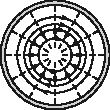
\includegraphics[height=5.35cm]{te01.pdf}
\caption{Radial magnetic field and azimuthal electric field of the $TE_{01}$ mode, adapted with permission from \cite{ramo}.}\label{fig:fc_te}
\end{figure}

A major contributor to the high accuracy of the method are the modes employed by the method. Like many other methods the split-cylinder uses circularly polarised transverse electric (TE) modes, so called TE\st{0n} modes. These modes are a group of field configurations that can exist inside a cylindrical waveguide and that have genuine advantages for dielectric measurements. Firstly, the TE\st{0n} modes of a cylindrical waveguide have the lowest attenuation coefficient of all cylindrical waveguide modes and unlike all other modes their attenuation monotonically decreases with frequency \cite{balanis}. The reason for this lies in the symmetry of the modes, due their azimuthal symmetry (i.e. $\vec{E}=E_{\phi}\vec{e}_\phi$) the magnetic field has only a axial component and radial component, of which only the component tangential to the waveguide walls, the $z$ component $H_z$, contributes to the losses in the waveguide walls. The $H_z$ component is inversely proportional to the frequency, making the attenuation losses along waveguide fall with frequency. Before the advent of modern fibre optical communications with their fundamental HE\st{11} mode and discovery of the near-IR low-loss window of silica, these modes were considered for microwave long-range communications. While cylindrical cavities not only have losses in the waveguide walls but also in the endplates that make up the cavity, they are still the modes with highest quality factors of all modes in cylindrical cavities. As can be seen in Fig. \ref{fig:q_cc} for the first few TE and TM modes, this is also true for most cylindrical waveguide geometries. This makes TE\st{0n} cavities very attractive for the measurement of low-loss dielectrics, since conductor losses are generally lower than in other cavities. The root cause for this is that for resonant dielectric loss measurements the dielectric loss becomes part of the energy balance that defines the quality factor.

\begin{equation}
Q=\frac{\omega_rW}{P_c+P_s} \qquad P_s = (\frac{\omega_rW}{Q}\pm u(\frac{\omega_rW}{Q}))-(P_c\pm u(P_c))
\end{equation}

To measure the dielectric loss, we need to determine the losses in the specimen $P_s$ from a measured resonant frequency and quality factor. We can model the fields in the cavity using appropriate mathematical techniques, which yields an estimate for the field configuration in the cavity. This estimate is then used to compute the energy $W$ in the entire cavity and in the specimen. To compute the losses in the cavity walls $P_c$, we take the  tangential magnetic field $\vec{H}_t$ on the cavity surface from the field configuration and compute the surface loss using the surface resistivity of the cavity walls. To accurately measure the dielectric losses in a cavity, we must accurately account for how much energy is dissipated in the cavity walls and how much is dissipated in specimen. For low-loss dielectrics the specimen loss $P_s$ becomes very small compared to the cavity loss $P_c$, so the uncertainty of the cavity loss estimate can easily dwarf the specimen loss, making the measurement of low-loss dielectrics less and less accurate. If the cavity loss is very low to begin with, the measurement is generally more accurate, reducing the influence of uncertainties arising from the field estimate or from the surface resistance estimate.

\begin{figure}
\centering
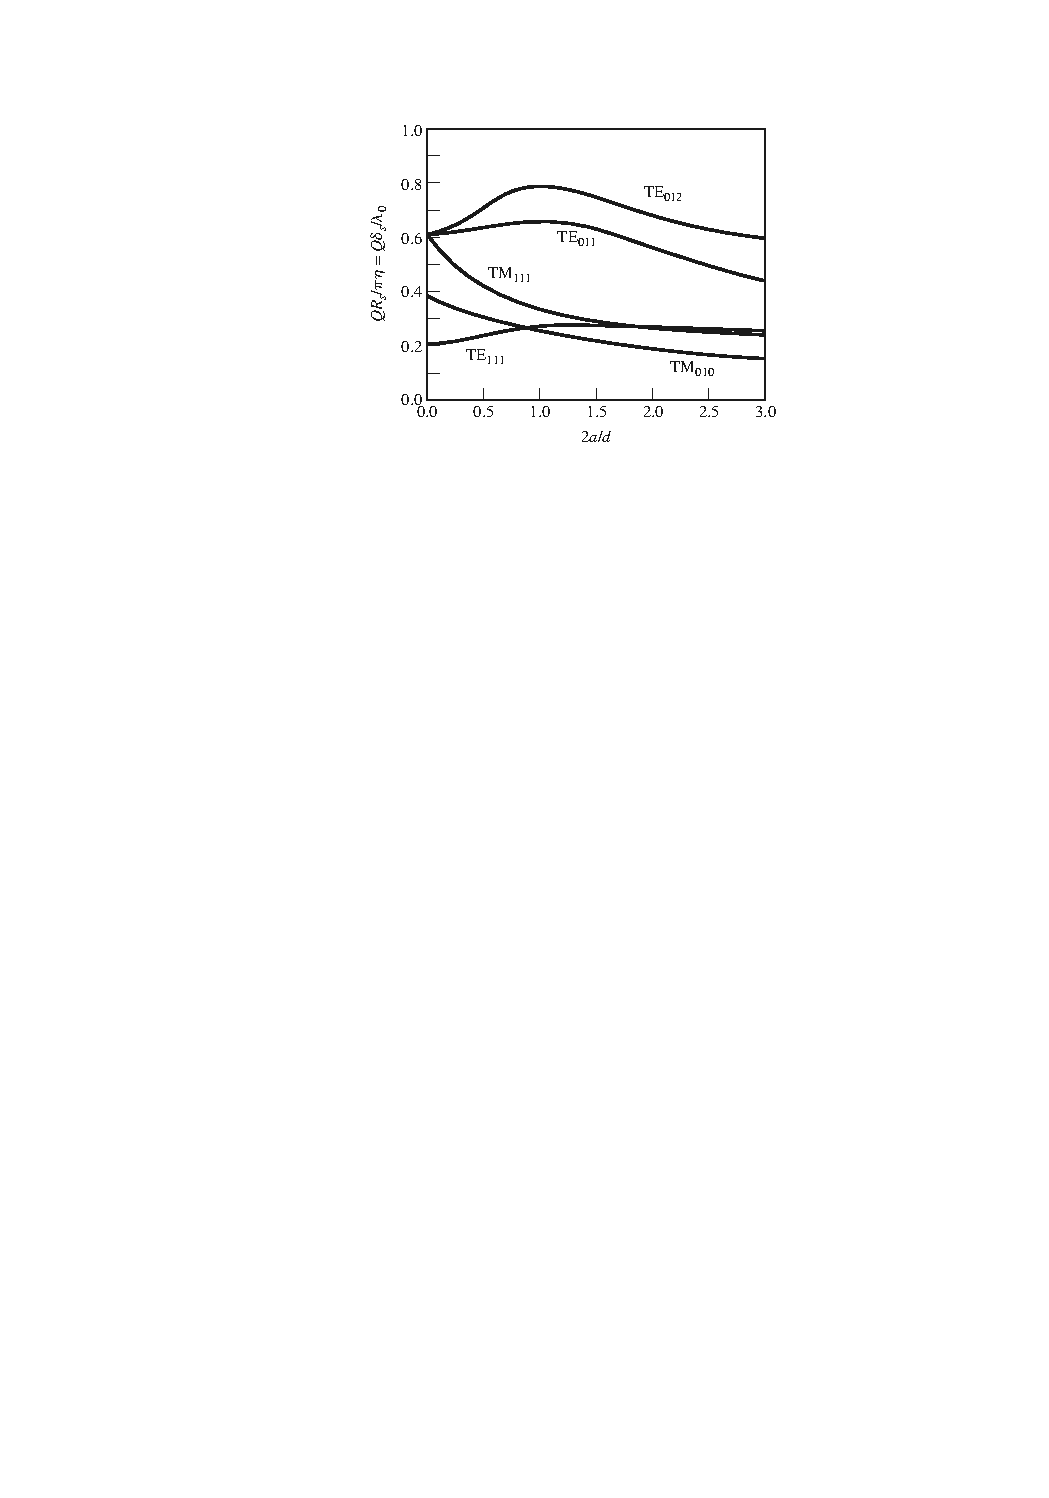
\includegraphics[height=0.27\textheight]{te_modes_q.pdf}
\caption{Normalized quality factors of cylindrical cavity modes for different cavity geometries, reproduced with permission from \cite{pozar}. $2a$ is the diameter of the cavity, and $d$ is the length. The dashed line marks the cavity geometry with the highest normalized quality factor.}\label{fig:q_cc}
\end{figure}

Secondly, the symmetry of the TE\st{0n} modes themselves has a positive influence on measurement accuracy. When measuring dielectrics in microwave cavities a major issue with many techniques are interfaces between dielectric and cavity walls and between dielectric and air. As these interfaces are typically not perfect, but random with numerous air-gaps scattered between the dielectric and the neighbouring material. If the electric field in the field region is perpendicular to these interfaces, the electric field becomes discontinuous and can cause systematic errors in dielectric measurements. Baker-Jarvis et al. \cite{tn1520} stated that measurement fixtures in which the electromagnetic fields are tangential to the air-material interface, such as TE\st{01} cavities and dielectric resonators, generally yield more accurate results than fixtures where the fields are normal to the interface. In the split-cylinder resonator the dielectric is placed in the middle of the resonator with its face directed into the direction of the axis of symmetry. A TE\st{0n} mode propagating from one end of the cavity to the other never encounters an interface where its electric field is normal to that interface, so air-gaps between the dielectric and cavity walls are effectively mitigated. Apart from this positive influence on measurement accuracy, the modes also simplify the measurement of thin materials. These materials typically only interact weakly with the cavity, so the measurement accuracy of thin materials is generally low. Tangential electric modes allow us to stack thin dielectrics hereby increasing the measurement accuracy \cite{NPL}.

Lastly, the field configuration is a good choice for the measurement of anisotropy in dielectrics. As we pointed out in our discussion of dielectric properties of materials at microwave frequencies, at the beginning of Chapter \ref{ch:methods}, many dielectric laminates as well as other materials have a weak anisotropy. These materials typically have different in-plane permittivities and out-of-plane permittivities. The circular polarisation of the mode allows us to directly determine the in-plane permittivity of these dielectrics or an average permittivity if the material is a weakly biaxial dielectric \cite{kent1996}. Unfortunately for many applications in microwave engineering the out-plane permittivity is more important, since the electric field orientation of many planar waveguides is predominantly normal to the surface of the material. To avoid this, two different different cavities can be used to characterise the dielectric, for example a TE\st{01} cavity may be used for the in-plane permittivity and a TM\st{010} cavity may be used for the out-of-plane permittivity \cite{dankov}.
\section{Coupling and Quality Factor Measurements of the Split-Cylinder Resonator}
The advantages of the TE\st{0n} modes has led to the development of various TE\st{01}-mode cavities \cite{NPL}, which are used for dielectric measurements of laminar low-loss dielectrics in the \SIrange{8}{40}{\giga\hertz} range. In this frequency range the microwave cavities can be easily manufactured and are not outperformed by open resonators, which are still relatively large at these frequencies. Many TE\st{01}-mode cavities are closed cavities with a uniform diameter and specimens cut to fit into the inside of the cavity. This simplifies the modelling of the cavities, but makes specimen preparation more complicated. While the split-cylinder resonator and all other TE\st{01}-mode cavities benefit from the TE\st{0n} modes, they also share two major disadvantages. The first disadvantage is that the TE\st{01} mode is not the dominant mode of the cylindrical cavity. Depending on the geometry of the cylindrical cavity, either the TM\st{010} mode or the TE\st{111} mode may be the dominant mode of a cylindrical cavity \cite[Sec. 9.3.2]{balanis}. To measure with TE\st{0n} modes we first need to identify the resonances of the TE\st{0n} modes in a measurement, for example in a transmission coefficient plot. Since the resonant frequencies of the modes depend on the geometry and the dielectric constant of the specimen, we need to estimate the dielectric constant before we can identify the TE\st{0n} modes. Janezic et al. \cite{janezicarz} found out that a fundamental TE\st{111} mode can be used to estimate the dielectric constant in a split-cylinder, but more on that topic later.

The second disadvantage of the TE\st{0n} modes are the degenerate TM\st{1n} modes. These modes are transverse magnetic modes (TM) that have the same dispersion relation as the TE\st{0n} modes, so their resonant frequencies are identical. The magnetic coupling loops of the split-cylinder resonator are used to suppress these degenerate modes. As we have already pointed out in Section \ref{sec:cofc}, the magnetic coupling loop couples only to modes that have magnetic field lines running through the loop. If we turn the face of the loop into the direction of $z$ axis of the resonator, i.e. the z-axis, all TM modes are effectively suppressed.

These modes have the same resonant frequency and a cavity has infinitely many modes with a wide range of different resonant frequencies. This raises the question, how can we measure a single resonance without interference from other modes? Coupling loops tap into all modes with field lines going through the loop. The equivalent circuit of a single loop (ref. Sec. \ref{sec:cofc}) are multiple ideal transformers in series with their secondary winding connected to resonant circuits, which make up the modes of the cavity. A split-cylinder resonator uses two coupling networks. Since the split-cylinder resonator is a measurement resonator, it is only weakly coupled to the rest of the measurement circuit. As have already mentioned, this keeps the modes in the resonator as undisturbed as possible and it allows us to directly measure the unloaded quality factor $Q_0$ of each mode. Unfortunately, reducing the coupling also makes the resonator highly resistive, so we need to use transmission-type quality factor measurements to keep the measurements accurate. Reflection coefficient measurements of highly resistive networks are known to be relatively inaccurate.
\begin{figure}
\centering
\begin{circuitikz}
\ctikzset {bipoles/length=0.9cm}

% Source network
\draw(-3,0) to[short] +(1.5,0)
			to[R=$Y_{01}$] +(0,-4.25);
\draw[dashed] (-1.5,-4.25) -- +(0,-1);
\draw(-1.5,-5.25) to[short] +(0,-2)
			to[short] +(-1.5,0)
			to[short] +(0,2);
\draw[dashed](-3,-5.25) -- +(0,1);
\draw(-3,-4.25)	to[I=$i_s$] +(0,4.25);

% Coupled resonator 1
\draw (0,0) to[short] +(0,-0.25)
			to[L,l_=$n_{11}$] +(0,-1.5)
			to[short] +(0,-0.5)
			to[open] +(0.5,2)
			to[short] +(1,0) node[above] {$Y_1$}
			to[fullgeneric,*-*] +(0,-1.5)
			to[open] +(0,1.5)
			to[short] +(1,0)
			to[open] +(0.5,-2)
			to[short] +(0,+0.5)
			to[L,l_=$n_{21}$] +(0,+1.5)
			to[short] +(0,+0.25)
			to[open] +(-0.5,-0.25)
			to[L,l_=$1$] +(0,-1.5)
			to[short] +(-2,0)
			to[L,l_=$1$] +(0,1.5)
			to[open] +(-0.45,-0.3)
			to [bend left] node[pos=0.5,above] {} ++(0.4,0)
			to[open] +(2.1,0)
			to [bend left] node[pos=0.5,above] {} ++(0.4,0);
			
% Coupled resonator 2
\draw (0,-2.25) to[short] +(0,-0.25)
			to[L,l_=$n_{12}$] +(0,-1.5)
			to[short] +(0,-0.25)
			to[open] +(0.5,1.75)
			to[short] +(1,0) node[above] {$Y_2$}
			to[fullgeneric,*-*] +(0,-1.5)
			to[open] +(0,1.5)
			to[short] +(1,0)
			to[open] +(0.5,-1.75)
			to[short] +(0,+0.25)
			to[L,l_=$n_{22}$] +(0,+1.5)
			to[short] +(0,+0.25)
			to[open] +(-0.5,-0.25)
			to[L,l_=$1$] +(0,-1.5)
			to[short] +(-2,0)
			to[L,l_=$1$] +(0,1.5)
			to[open] +(-0.45,-0.3)
			to [bend left] node[pos=0.5,above] {} ++(0.4,0)
			to[open] +(2.1,0)
			to [bend left] node[pos=0.5,above] {} ++(0.4,0);
% Dashed line
\draw[dashed] (0,-4.25) -- +(0,-1);
\draw[dashed] (3,-4.25) -- +(0,-1);
% Coupled resonator 3
\draw (0,-5.25) to[short] +(0,-0.25)
			to[L,l_=$n_{1N}$] +(0,-1.5)
			to[short] +(0,-0.25)
			to[open] +(0.5,1.75)
			to[short] +(1,0) node[above] {$Y_N$}
			to[fullgeneric,*-*] +(0,-1.5)
			to[open] +(0,1.5)
			to[short] +(1,0)
			to[open] +(0.5,-1.75)
			to[short] +(0,+0.25)
			to[L,l_=$n_{2N}$] +(0,+1.5)
			to[short] +(0,+0.25)
			to[open] +(-0.5,-0.25)
			to[L,l_=$1$] +(0,-1.5)
			to[short] +(-2,0)
			to[L,l_=$1$] +(0,1.5)
			to[open] +(-0.45,-0.3)
			to [bend left] node[pos=0.5,above] {} ++(0.4,0)
			to[open] +(2.1,0)
			to [bend left] node[pos=0.5,above] {} ++(0.4,0);

% Connection networks
\draw (-1.5,0) to[short,*-] +(1.5,0);
\draw (-1.5,-7.25) to[short,*-] +(1.5,0);
% Load network
\draw (3,0) to[short] +(1.5,0)
			to[R=$Y_{02}$] +(0,-4.25)
			to[open] +(0,-1)
			to[short] +(0,-2)
			to[short] +(-1.5,0);
\draw[dashed] (4.5,-4.25) -- +(0,-1); 

% Resonant circuit
\draw (6,-2) to[fullgeneric=$Y_n$,o-o] +(0,-2);
\draw[double, latex-latex] (7,-3) to +(1.5,0);

\draw (10,-4.25) to[short,o-] +(0,+0.5)
			to[short] +(1,0)
			to[C,l_=$C_n$] +(0,1.5)
			to[short,-*] +(-1,0)
			to[short] +(-1,0)
			to[R=$R_n$] +(0,-1.5)
			to[short,-*] +(1,0)
			to[L,l_=$L_n$] +(0,1.5)
			to[short,-o] +(0,+0.5);


\end{circuitikz}
\caption{Equivalent circuit of the Split-Cylinder resonator.}\label{fig:splitc_model}
\end{figure}
To model the filtering of unwanted TM modes and the interference from neighbouring modes, we can use the equivalent circuit of the split-cylinder resonator of Fig. \ref{fig:splitc_model}. The circuit uses ideal transformers in series at the input and the output of the resonator, which all have RLC resonant circuits on their secondary winding. Unlike the equivalent circuit of the coupling loop that we discussed in Sec. \ref{sec:cofc}, this resonator is under-coupled, so the self-inductances of both loops become negligible. The resonant circuits and the ideal transformers remain. The coupling coefficient of each ideal transformer depends on the magnetic field strength of the mode on its secondary winding. TM modes and also TE modes with a field minimum along the z-axis have very small coupling coefficients. 

The result of a transmission-type quality factor measurement of a split-cylinder resonator is a transmission coefficient plot that is a superposition of all modes that couple to the coupling loop. The resonance condition of such a resonator is unlike that of a simple RLC resonant circuit. An accurate measurement of the resonant frequency and the quality factor of a mode is only possible if the measurement mode is the only mode oscillating in a certain frequency range. We can calculate the transmission coefficient of the equivalent circuit of Fig. \ref{fig:splitc_model} to get an expression for the superposition of all modes
\begin{equation}\label{eq:s_modes}
S_{21}(\omega)=\frac{2\sqrt{Y_{01}Y_{02}}\left(\sum\limits_{n=1}^{N}\frac{n_{1n}n_{2n}}{Y_n}\right)}{1+\sum\limits_{n=1}^{N}\left(\frac{n_{1n}^2Y_{01}}{Y_n}+\frac{n_{2n}^2Y_{02}}{Y_n}\right)+\sum\limits_{n=1}^{N}\sum\limits_{\substack{k=1 \\ n\neq k}}^{N}\frac{Y_{01}Y_{02}\left(n_{1n}n_{2k}-n_{2n}n_{1k} \right)^2}{Y_nY_k}} \text{,}
\end{equation}
where
\begin{equation}
Y_n(\omega)=G_{0,n}(1+jQ_{0,n}\delta_n) \quad \text{and} \quad \delta_n = \frac{\omega}{\omega_{r,n}}-\frac{\omega_{r,n}}{\omega}\text{.}
\end{equation}
Using Eq. \eqref{eq:s_modes} we can show that multiple modes may be resolved through careful fitting or that individual modes may be measured if they are undisturbed, i.e. do not overlap with neighbouring modes. In our measurements with the split-cylinder resonator we decided to use only undisturbed modes to simplify the matter. An undisturbed mode requires all neighbouring modes to have either minuscule coupling like in the case of the degenerate TM modes ($n_{1n}\rightarrow 0$ or $n_{2n}\rightarrow 0$) or a relatively small bandwidth of the resonance curve so that we can assume $Y_n\rightarrow\infty$ for all neighbouring modes in the vicinity of the mode. In these two cases Equation \eqref{eq:s_modes} simplifies to
\begin{equation}
S_{21}(\omega)=\frac{2\sqrt{n_{11}^2Y_{01}n_{21}^2Y_{02}}}{n_{11}^2Y_{01}+n_{21}^2Y_{02}+G_{0,1}(1+jQ_{0,1}\delta_1)}\text{,}
\end{equation}
which is the same result as in the case of the transmission-type measurement of a single RLC resonant circuit.(cf. Eq. \eqref{eq:tr_S}) This proves that a single mode can be accurately measured as long as the mode is undisturbed.

For these derivations we assumed that the resonator was very under-coupled. This implied that the inductance of the coupling loop became negligible, so the inductive loading of the resonator disappeared. In our measurements we also observed that the resonant frequency converged to a constant value when we reduced the coupling. The resistive loading on the other hand did not disappear, since we still need to couple power through the resonator for our measurements! Resistive loading has the downside that it changes the quality factor, so our assumption that the loaded quality factor is equal to the unloaded quality factor is not entirely valid. There is a trade-off between having enough coupling to accurately measure a resonance curve, and keeping the coupling weak enough to ensure $Q_L\approx Q_0$. Janezic \cite{janezic} suggested that a peak transmission coefficient of less than \SI{-50}{\decibel} was a good compromise between the two criteria. In our measurements we found that a coupling level of \SIrange{-70}{-50}{\decibel} was often a good choice. At these coupling levels we can show for symmetric coupling
\begin{equation}
n_{11}^2Y_{01}=n_{21}^2Y_{02}=Y'
\end{equation}
\begin{equation}
S_{21}(\omega)=\frac{2\sqrt{n_{11}^2Y_{01}n_{21}^2Y_{02}}}{n_{11}^2Y_{01}+n_{21}^2Y_{02}+G_{0,1}(1+jQ_{0,1}\delta_1)}=\frac{\frac{1}{1+\frac{G_{0,1}}{2Y'}}}{1+j\frac{Q_{0,1}\delta_1}{1+\frac{2Y'}{G_{0,1}}}}\text{.}
\end{equation}
If we take the peak coupling levels of our measurements, we yield the coupling coefficient
\begin{equation}
S_{21}(\omega_r)=\frac{1}{1+\frac{G_{0,1}}{2Y'}} \Rightarrow \frac{2Y'}{G_{0,1}}=2\kappa=\frac{1}{\frac{1}{S_{21}(\omega_r)}-1}=\num{3.16e-4}\ ...\ \num{3.17e-3}
\end{equation} 
and the unloaded quality factor 
\begin{equation}
Q_0=(\num{1.00032}\ ...\ \num{1.00317})Q_L
\end{equation} of the resonator at these levels. Thus, we have shown that the coupling coefficient has a small influence on our quality factor measurements, but as we will see when discuss our measurement results the influence of the coupling is generally negligible. 
\section{Modelling the Split-Cylinder Resonator}\label{sec:modelling}
In this section we now address the electro-magnetic modelling of the split-cylinder resonator. Ermert \cite{ermert}, Guillon \cite{guillon}, Koba\-yashi \cite{kobayashi} and Kent \cite{kent1996} were among the first to analyse the split-cylinder resonator. Kent developed a split-cylinder resonator that he called resonant dielectrometer, which built on the available research in the area of TE\st{0n} cavities. He used coupling loops to suppress the degenerate TM modes. He proposed to measure the permittivity by at first modelling the cavity as a closed cavity with uniform diameter and then correcting the error of the model with a gap correction. The permittivity of a sample in a closed cavity was computed using a simple Eigenvalue problem and the gap correction was derived from a perturbation calculation. \cite{kent1996gap} Kobayashi used a very similar model, although he computed a gap-correction using a Rayleigh-Ritz method and suggested using a PTFE ring in the cavity as a mode filter for the degenerate TM\st{11} modes.

Janezic \cite{janezic1999} later derived a full-wave model of the split-cylinder resonator. Like the other authors he recognised that the boundary value problem extends into the outside of the cavity and proposed an infinitely large sample radius as an approximation for this boundary value problem. The sample was supposed to backed by a infinitely large flange confining all the fields to the sample and the cavity. For the modes he assumed that TE\st{0n} modes excite only TE\st{0n} modes and that the modes in the cavity can be represented by a series expansion of TE\st{0n} modes. He used a Hankel transform to solve the field problem and showed that the approximation is correct for relatively large, thin specimens. Although convergence was achieved with a small number of modes, the wall losses were omitted in the model to limit computational complexity. 

For his PhD thesis Janezic \cite{janezic} studied the split-cylinder resonator in detail and compared three theoretical models for the resonator. The three models were a mode-matching model, a least-squares boundary residual model (LSBR) and a Hankel-transform model. For the mode-matching and the LSBR model he modelled the the cavity as a closed cavity with a perfectly conducting boundary at $\rho=b$ in the sample region and a perfectly conducting flange ranging from the cavity diameter to the the perfectly conducting boundary at $\rho=b$. He recognised that this assumption simplified the calculations greatly and led only to a small systematic error in the measurements. His Hankel transform model used the same boundary conditions as his original model \cite{janezic1999}, so he also assumed an infinitely large sample radius and an infinitely large flange. Unlike in his original model the loss calculations of all models also included the losses of the cavity. He compared all three models in terms of the satisfaction of boundary conditions, the accuracy of the measured relative permittivity, the accuracy of the measured loss tangent and the computational speed of the model. The mode-matching model was selected as the best model, because it was the fastest model and also computed the complex permittivity accurately. As far as the other methods were concerned, the least-squares boundary residual model was found to be fast, but the accuracy of the computed permittivities was generally poor due to problems with the weighing functions of the model. The Hankel transform model showed some potential, but the computation of the Hankel transforms was very slow and the loss calculations neglected the flange loss due to problems with the numerical integration of a Hankel transform. Janezic also made a few measurements with the mode-matching model in which the model generally performed very well. He also added a uncertainty calculation for the mode-matching model.

The convenience and accuracy of the split-cylinder method has also gained the interest of the circuit board and dielectric substrate industry. This has led to the standardisation of Kobayashi's model and of Janezic's mode-matching model. Kobayashi's model was first standardised in 2002 as Japanese standard JIS R 1641 \cite{kobayashistandard} and subsequently in 2011 as IEC standard IEC 62562 \cite{iecSC}. The mode-matching model was standardised in 2007 as IPC test method TM-650 2.5.5.13 \cite{ipcSC}. Keysight \cite{keysightSC} also implemented a split-cylinder resonator based on Janezic's mode-matching model.

Recently two new models for the split-cylinder resonator were published, which both aimed at improving the mode identification of the split-cylinder resonator. Although the mode-matching model and the other models are very accurate and well understood, they only calculate the TE\st{0np} modes of the resonator. As we have already mentioned before, the TE\st{011} mode is not the dominant mode of the resonator, so one approach is to estimate the dielectric constant from the dominant TE\st{111} mode and then calculate the resonant frequency of the higher modes from this estimate. The calculated resonant frequencies are in turn used to find the resonant frequencies in our measurements and compute the actual dielectric constant \cite{janezicarz}. This approach is acceptable as long as the dielectric constant varies only slowly over frequency, which is the case for all low-loss dielectric (cf. Chapter \ref{ch:methods}), and as long as only one resonance of transmission coefficient lies close to the calculated resonant frequency. If more than one resonance curve lies close to the calculated resonant frequency, this method fails. A model for all TE and TM modes would allow us to identify all modes, even if two modes lie very close to each other. For this purpose Zinal \cite{zinal} proposed an extended mode-matching model, which included all TE and TM modes. Since he neglected the fringing fields in his calculations, the model was less accurate than others models. Villaroya \cite{villaroya1,villaroya2} also published a model for all TE and TM modes. His model used a full-wave circuit method that also used the same boundary conditions as Janezic's mode-matching model. In his article he only used TE\st{0np} modes for his complex permittivity measurements, since he recognised that the uncertainty of $\tan\delta$ measurements with other TE modes was generally too high. He published his model only a few months before the publication of this thesis, so it still remains to be seen whether his model can both accurately measure the TE\st{0np} modes and identify all modes of split-cylinder resonator.
